\section{Illicit Address Detection}


\subsection{Dataset}
\textbf{Scam addresses}

The scam addresses used for detection are the 6,004 scam addresses collected from the money-flow analysis.

\textbf{Licit addresses}
We collected 6,014 addresses from WalletExplorer.com\cite{walletexplorer}, a bitcoin blockchain explorer which merges addresses together. The address clusters are labelled as exchanges, pools, services, gambling, etc. It also identifies the specific service name, such as for exchanges there are huobi.com\cite{huobi},Bittrex.com\cite{bittrex}, for pools there is SlushPool.com\cite{slushpool}.

\textbf{Unknown addresses}
Based on the two parts of data above, we expended the dataset to a further layer in the graph. We firstly found out all of the transactions related to the nodes from explorer.bitcoin.com\cite{explorer.bitcoin.com}, the process is demonstrated in \ref{fig:1-layer-data-expand} then we collected the transaction detail information from btc.com\cite{btc.com}. Figure\ref{fig:2-layer-data-expand} illustrates the second layer expansion of the dataset. The transaction detail will include the input and output addresses of each transaction, which lead us to accomplish the dataset expansion.
\begin{figure}[tbp]
\centerline{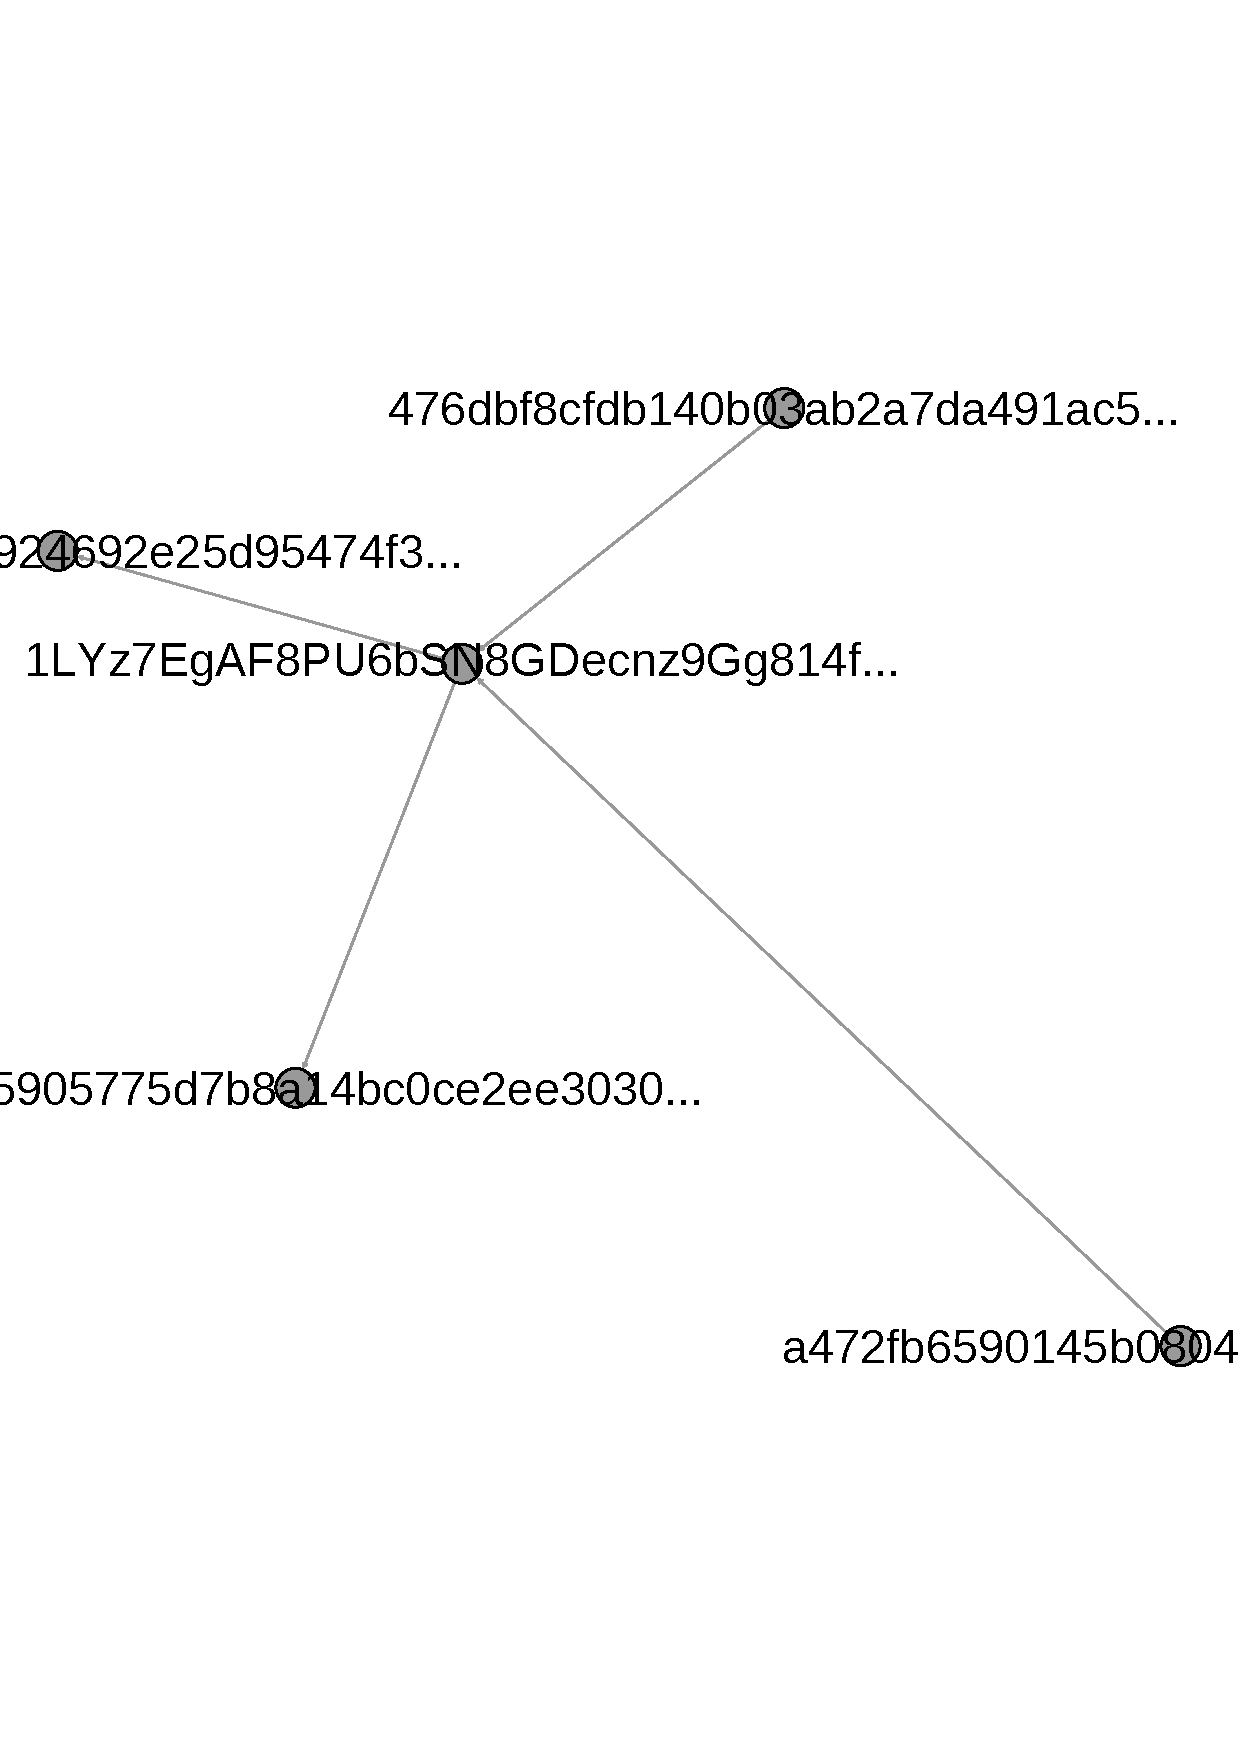
\includegraphics[width=0.6\columnwidth]{images/1-layer-data-expand.pdf}}
\caption{Find transactions for labelled address}
\label{fig:1-layer-data-expand}
\end{figure}
\begin{figure}[tbp]
\centerline{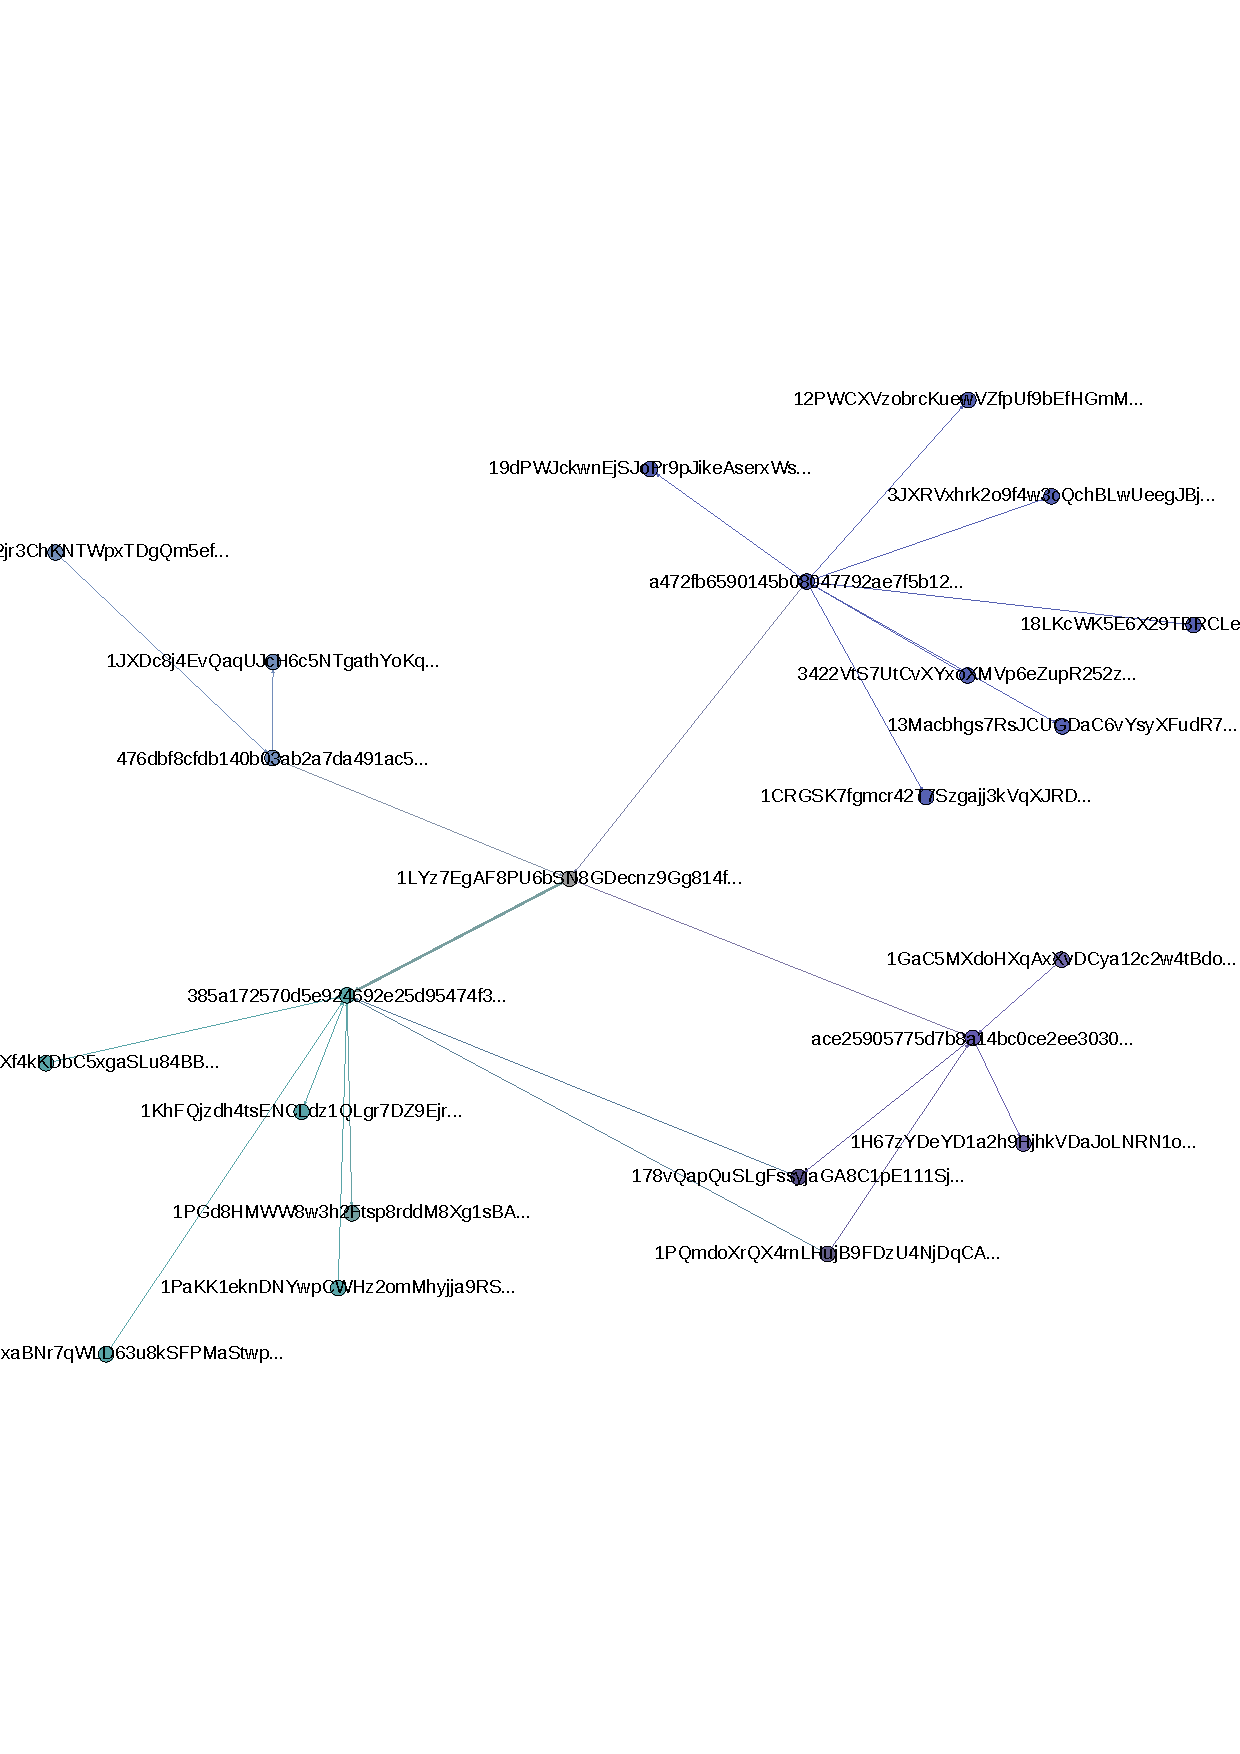
\includegraphics[width=\columnwidth]{images/2-layer-data-expand.pdf}}
\caption{Find 2nd layer data}
\label{fig:2-layer-data-expand}
\end{figure}

Finally, there are 6,004 scam addresses, 6,014 licit addresses. Besides these 12,018 labelled addresses, there are 4,754,462 unlabelled nodes. These nodes are linked together with 56,772,062 in an undirected graph.


\subsection{Feature Extraction}
\label{sec:feature-extraction}
At first, we are going to extract features for further classification. The features of addresses used in our classification are summarized in table \ref{table:feature-extraction}, 8 statistics refer to summation, average, median, maximum, minimum, standard deviation, kurtosis, and skewness of the corresponding feature.

The feature extracted can be divided into two parts, the first part related to the addresses, the second part related to incoming and outgoing transactions of the addresses. The lifetime of an address refers to the time period between the first transaction and last transaction. The seond part features are some transaction related features. Such as transaction fees, Block weight, etc.

From table\ref{table:feature-avg} we can tell that the chosen features has an obvious difference between the scam addresses and the illicit addresses.


\begin{table}[htbp]
 \caption{Feature Extraction\label{table:feature-extraction}}
 \begin{tabularx}{80mm}{c|>{\centering\arraybackslash}X>{\centering\arraybackslash}X}
  \toprule
 \textbf{Feature Type}& \textbf{Extracted Feature}& \textbf{Extracted Distributions} \\
  \midrule
 Addresses & Lifetime & -\\
\multirow{11}{*}{ Transactions} & Transaction Fee& 8 statistics \\
 & Transaction fee rate \newline (BTC/KvB)& 8 statistics \\
 & Block Weight & 8 statistics \\
 & Incoming Address Number & 8 statistics\\
 & Outgoing Address Number & 8 statistics\\
 & Input Volume & 8 statistics\\
 &Output Volume & 8 statistics\\
 & Confirmation& 8 statistics \\
 & Sigops &  8 statistics \\
 & Size(Bytes)& 8 statistics\\
 & Virtual size(Byte)& 8 statistics \\ 
  \bottomrule
 \end{tabularx}
\end{table}

\subsection{Approach}
As for the neural network. Here we prepare two sets of dataset, which are labeled neural network 1 and neural network 2. 

\textbf{Traditional Machine Learning}
Neural network 1 aims at implementing a supervised neural network classification. Neural network1 consists of all the labelled node, i.e. 6,014 licit addresses and 6,004 scam addresses. All of the features extracted in \ref{sec:feature-extraction} is going to be implemented when training and testing this neural network.

\textbf{Graph Neural Network}
As there are a huge part of addresses in our dataset without label, in building neural network 2 we aims at implementing semi-supervised neural network classification. This net can not handle too many features, which may greatly slow down the training speed and has a higher hardware requirement. So we choose three topological features for each node: degree, in-degree, out-degree. This graph consist of 12,018 labelled nodes and 4,754,462 unlabelled nodes. The graph is undirected with 56,772,062 edges.
\begin{table}[htbp]
\centering
 \caption{Average feature value\label{table:feature-avg}}
 \begin{tabular}{lcl}
  \toprule
 Extracted Feature& Avg-1\footnote{The average value for the corresponding feature among the whole scam address dataset} & Avg-2\footnote{The average value for the corresponding feature among the whole illicit address dataset} \\
  \midrule
 Lifetime & 99.6673& 54.3247\\
  Transaction fee rate & 0.0011 & 0.006\\
  Block Weight & 0.0006 & 0.0007\\
  Incoming Address Number & 16.7196&93.4668 \\ 
  Outgoing Address Number& 11.4008& 109.8912\\ 
  Input Volume& 15.5606& 39.9797\\
  Output Volume& 15.5663& 39.9821\\ 
 Confirmation & 77405.5936&145133.932 \\
   Sigops& 2453.8119& 12506.3434\\
  Size(Bytes)& 9814.3251& 50024.4237\\
  Virtual size(Byte)& 40.3983&276.7595 \\
  

  \bottomrule
 \end{tabular}
\end{table}


\subsection{Experiments}
We splited the dataset into training, test and validation data in 6:2:2 way. We firstly tested standard classification models for the scam and illicit prediction using some standard classifier. The parameters setting is shown in table\ref{table:classifier-parameter}, those parameters that are not specified in this table is implemented using the value defaulted in scikit-learn\cite{pedregosa2011scikit}.
\begin{table}[htbp]
\centering
 \caption{Parameters for classifier\label{table:classifier-parameter}}
 \begin{tabularx}{0.3\textwidth}{XX}
  \toprule
 Classifier&  Parameter \\
  \midrule
 Logistic Regression & solver=`liblinear', max\_iter=500\\
 SVM & C=10, kernel=`linear' \\
  KNN & n\_neighbors=50\\
  MLP & max\_iter=1000, solver=`sgd', hidden\_layer\_sizes=50 \\ 
  Ramdom Forest & n\_estimators=30, max\_depth=200,  min\_weight\_fraction\_leaf=0.2\\ 
  \bottomrule
 \end{tabularx}
\end{table}

We evaluate these models by using all the 89 features, except for neural network2. In neural network2 we only consider 3 topological features. The standard methods result and the neural network result is shown in table \ref{table:classifier-result}.

\begin{table}
\centering
 \caption{Classification result\label{table:classifier-result}}
    \begin{tabularx}{0.49\textwidth}{>{\centering\arraybackslash}X|ccccc}
		\hline \textbf{Classifier} & \textbf{precision}  &\textbf{AUC} & \textbf{accuracy} &\textbf{recall}&\textbf{F1-score}\\
		 \hline Logistic    Regression & 0.9773& 0.9786 & 0.9516 & 0.9276 & 0.9479\\
		 SVM & 0.9968  & 0.9974 & 0.9849 &0.9839 &0.9782\\  
		 NCA & 0.9931& 0.9944 & 0.9649 & 0.9581 & 0.9628\\
		 MLP &0.9946 & 0.9964 &0.9852 & 0.9795& 0.9840\\
		 Random Forest & 0.9799& 0.9817 & 0.9352 &0.9323 &0.9303 \\
		 nn1 GCN & 0.9395 & 0.9772 & 0.9363 & 0.9340 & 0.9368 \\
         nn2 GCN & 0.7357& 0.7685& 0.7706&0.8609 & 0.7934\\


	     \hline
    \end{tabularx}
\end{table}

From this table we can find out that the traditional classifiers all have precision higher than 97\%, GCN works well in neural network 1, but works poorly in neural network 2. The result indicates that the semi-supervised GCN is still not good enough to perform classification based on our dataset to do the classification. The reason may be because the features chosen are not sufficient.

\noindent\fbox{
\begin{minipage}{0.47\textwidth}{
\textbf{Answer to RQ4}: \textit{We explorer classification methods in our dataset. Logistic Regression, SVM, KNN, MLP are used here as benchmark method, we also implement GCN both in supervised and semi-supervised ways. We constructed two neural network here. The result shows that except for the semi-supervised classification, other methods can reach precision higher than 93\%.}
}\end{minipage}}
